\begin{figure}[t]
  %%% Scenario 1 %%%
  \centering
  \begin{subfigure}[b]{0.32\textwidth}
    \centering
    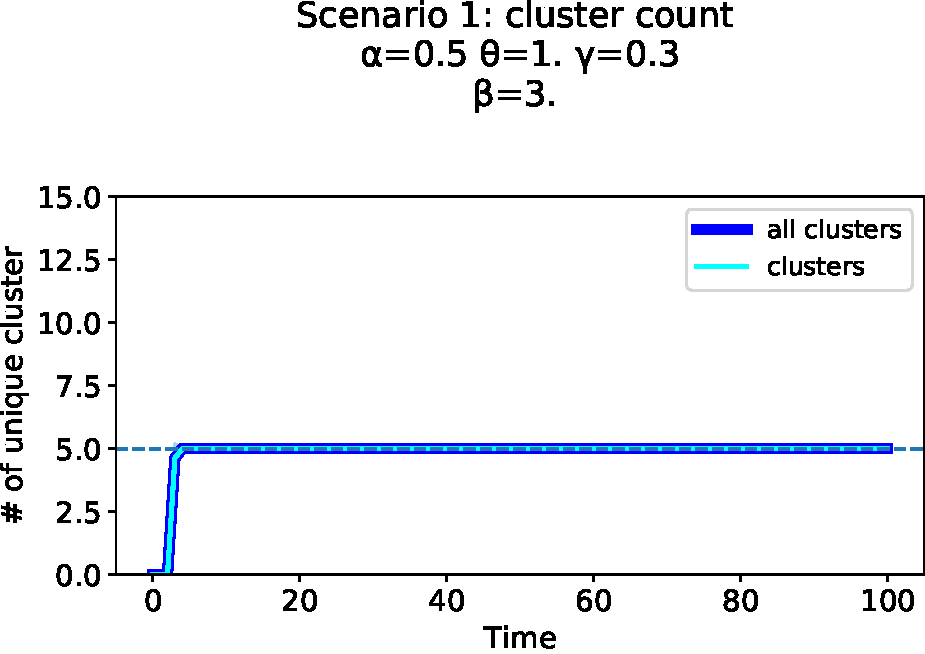
\includegraphics[width=\textwidth]{papers/swarm-intelligence2021/img/simulations/standard_cluster_count.pdf}
  \end{subfigure}
  \hfill
  \centering
  %%% Scenario 2 %%%
  \begin{subfigure}[b]{0.32\textwidth}
    \centering
    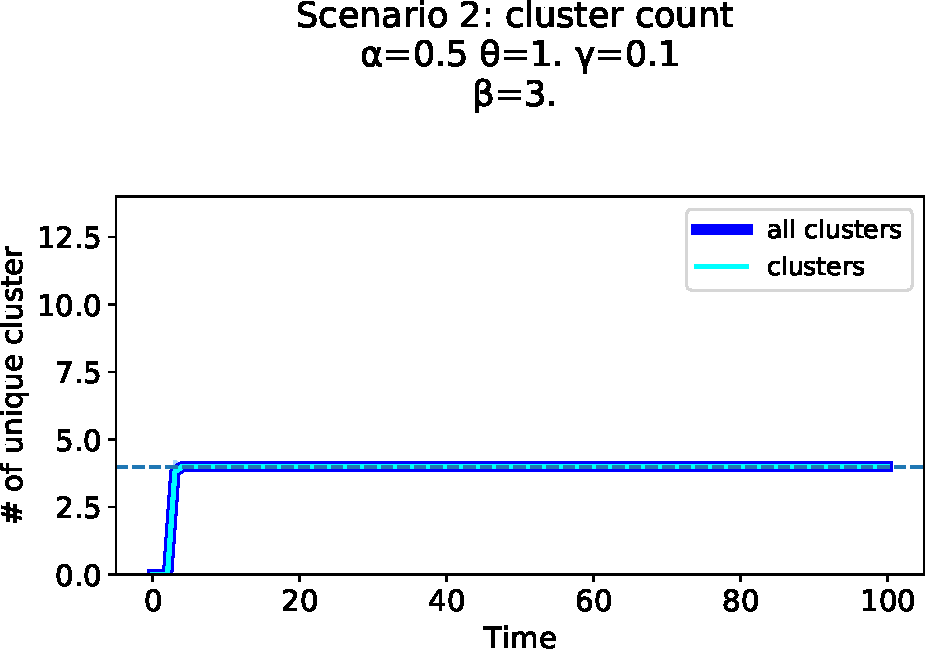
\includegraphics[width=\textwidth]{papers/swarm-intelligence2021/img/simulations/stretched_cluster_count.pdf}
  \end{subfigure}
  \hfill
  \centering
  %%% Scenario 3 %%%
  \begin{subfigure}[b]{0.32\textwidth}
    \centering
    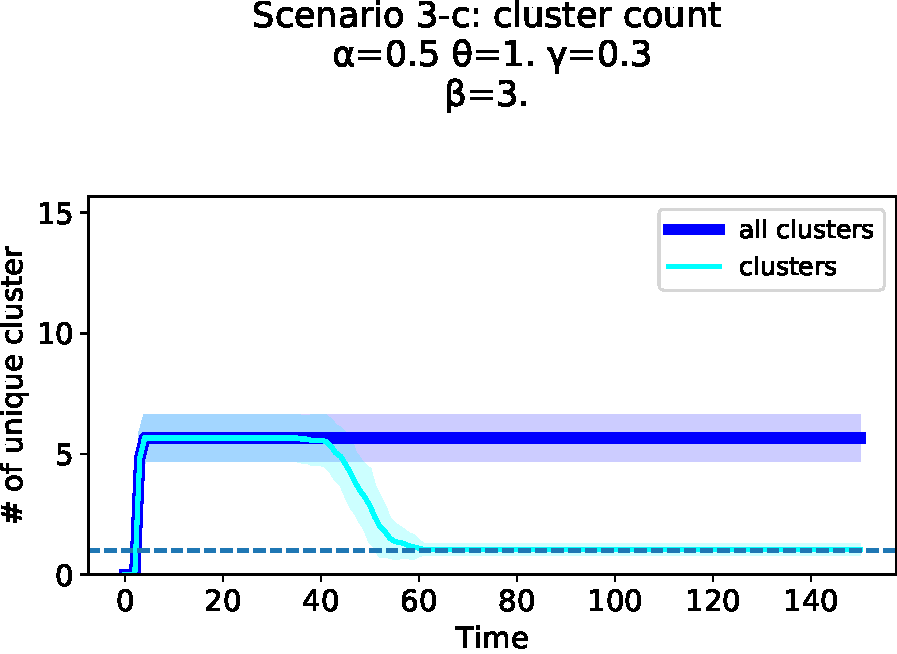
\includegraphics[width=\textwidth]{papers/swarm-intelligence2021/img/simulations/one-direction_0_021_α-0.5_θ-1._γ-0.3_β-3._ω-0._ζ-0..pdf}
  \end{subfigure}
  \hfill
  \centering
  %%% Scenario 4 %%%
  \begin{subfigure}[b]{0.32\textwidth}
    \centering
    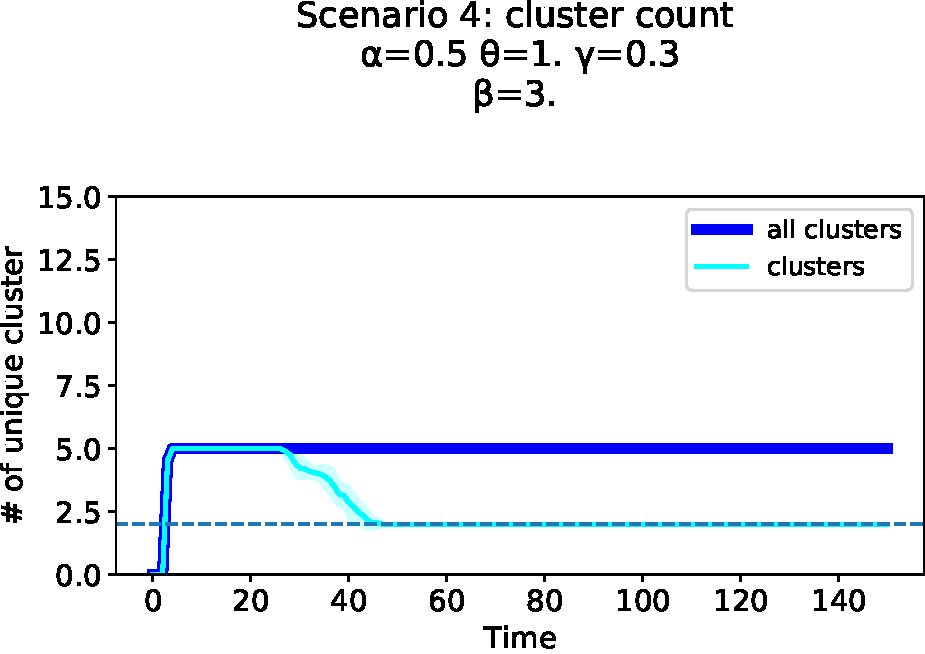
\includegraphics[width=\textwidth]{papers/swarm-intelligence2021/img/simulations/overlay_0_021_α-0.5_θ-1._γ-0.3_β-3._ω-0._ζ-0..pdf}
  \end{subfigure}
  \hfill
  \centering
  %%% Scenario 5 %%%
  \begin{subfigure}[b]{0.32\textwidth}
    \centering
    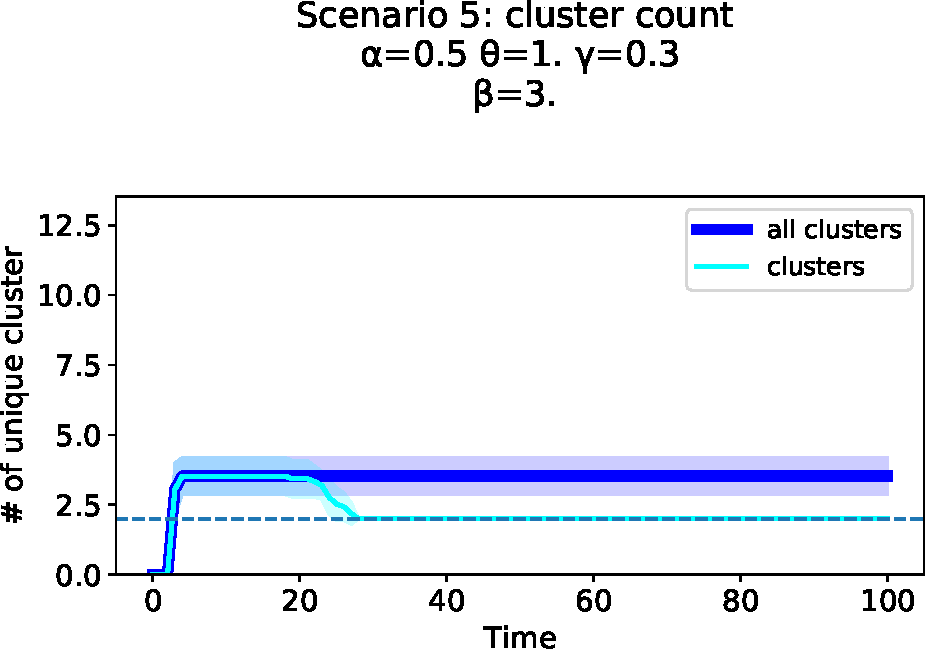
\includegraphics[width=\textwidth]{papers/swarm-intelligence2021/img/simulations/non-convex_0_021_α-0.5_θ-1._γ-0.3_β-3._ω-0._ζ-0..pdf}
  \end{subfigure}
  \hfill
  \centering
  %%% Scenario 6 %%%
  \begin{subfigure}[b]{0.32\textwidth}
    \centering
    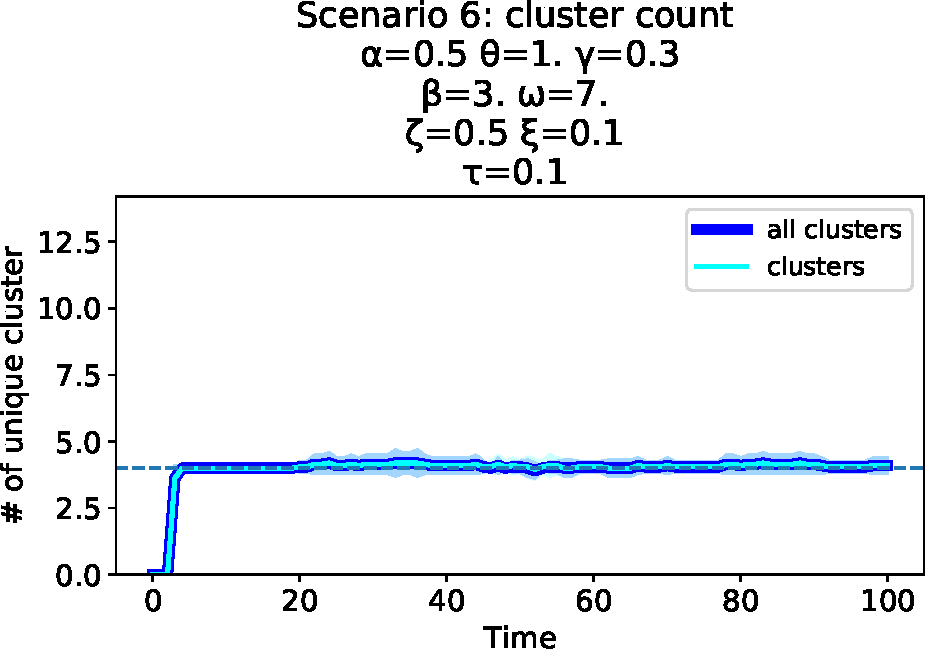
\includegraphics[width=\textwidth]{papers/swarm-intelligence2021/img/simulations/movement_cluster_count.pdf}
  \end{subfigure}
  \centering
  %%% Scenario 7 %%%
  \begin{subfigure}[b]{0.32\textwidth}
    \centering
    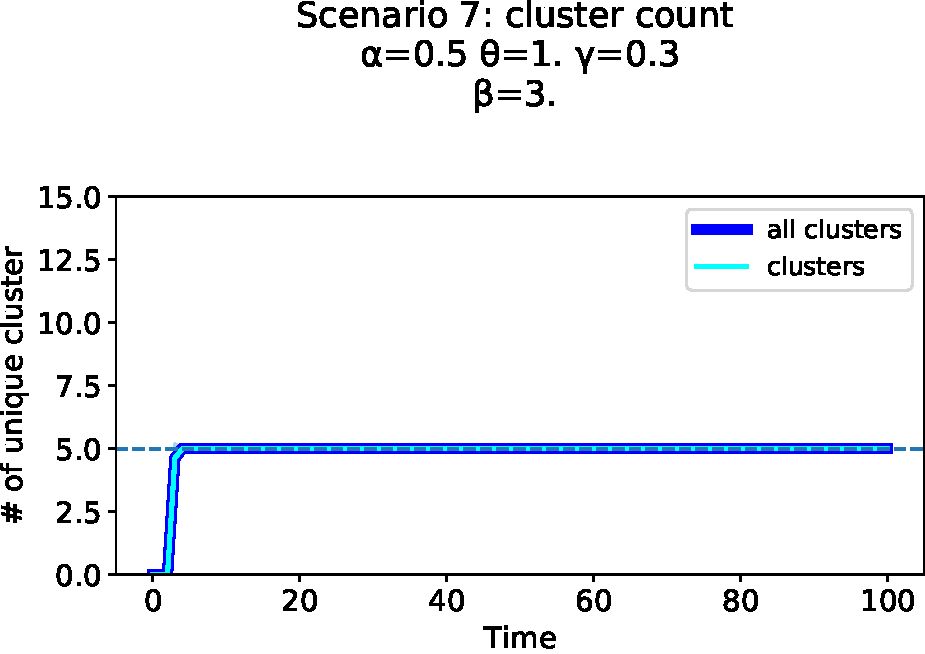
\includegraphics[width=\textwidth]{papers/swarm-intelligence2021/img/simulations/standard-updatable_0_021_α-0.5_θ-1._γ-0.3_β-3._ω-0._ζ-0..pdf}
  \end{subfigure}
  %%% Scenario 8 %%%
  \begin{subfigure}[b]{0.32\textwidth}
    \centering
    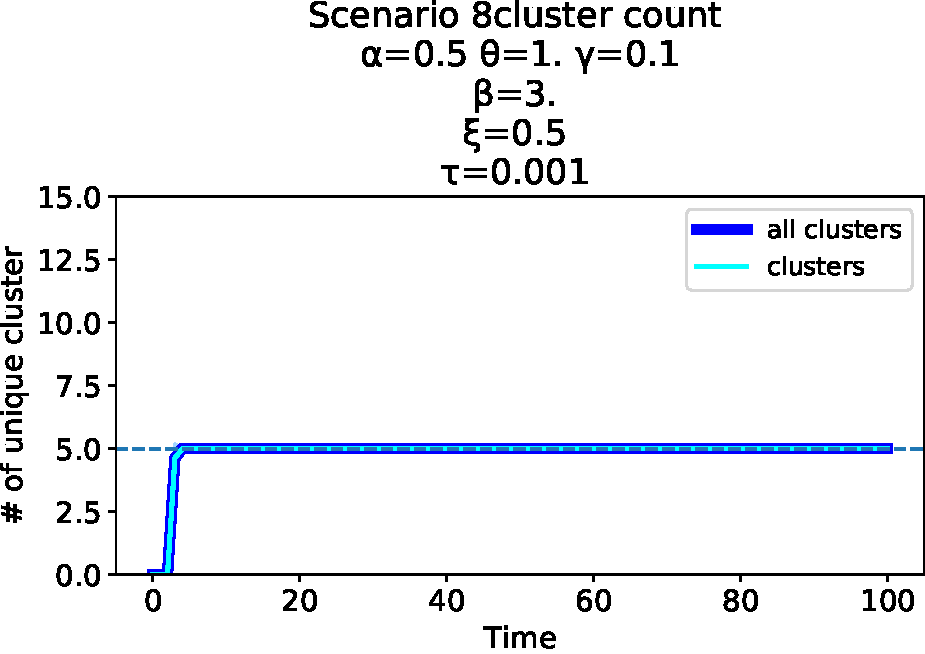
\includegraphics[width=\textwidth]{papers/swarm-intelligence2021/img/simulations/failScenario_0_021_α-0.5_θ-1._γ-0.1_β-3._ω-0._ζ-0._ξ-0.5_τ-0.001}
  \end{subfigure}
  \caption[Overview of simulation results in different clustering scenarios]{Overview of simulation results. 
  The dotted lines identify the ideal cluster division count. 
  The blue lines show the unique cluster found. 
  Instead, the cyan lines indicate the unique cluster number after the merging phase. 
  %In each scenario, the algorithm eventually reaches the correct cluster division count. 
  }
  \label{fig:overview-results}
\end{figure}